%
% File acl2014.tex
%
% Contact: koller@ling.uni-potsdam.de, yusuke@nii.ac.jp
%%
%% Based on the style files for ACL-2013, which were, in turn,
%% Based on the style files for ACL-2012, which were, in turn,
%% based on the style files for ACL-2011, which were, in turn, 
%% based on the style files for ACL-2010, which were, in turn, 
%% based on the style files for ACL-IJCNLP-2009, which were, in turn,
%% based on the style files for EACL-2009 and IJCNLP-2008...

%% Based on the style files for EACL 2006 by 
%%e.agirre@ehu.es or Sergi.Balari@uab.es
%% and that of ACL 08 by Joakim Nivre and Noah Smith

\documentclass[11pt]{article}
\usepackage{acl2014}
\usepackage{times}
\usepackage{url}
\usepackage{latexsym}
\usepackage{graphicx}
\usepackage{amsmath}
\usepackage[]{algorithm2e}
\usepackage{caption}
\usepackage{subcaption}

\DeclareGraphicsExtensions{.pdf,.png,.jpg}

%\setlength\titlebox{5cm}

% You can expand the titlebox if you need extra space
% to show all the authors. Please do not make the titlebox
% smaller than 5cm (the original size); we will check this
% in the camera-ready version and ask you to change it back.


\title{High-Dim Project}

\author{Chris Kedzie \\
  Columbia University\\
  {\small \tt kedzie@cs.columbia.edu} \\\And
  Dahong Liu \\
  Columbia University\\
  {\small \tt dl2868@columbia.edu} \\\And
  Xiao Zhu\\
  Columbia University\\
  {\small \tt xz2362@columbia.edu} \\\And
  Yichi Zhang\\
  Columbia University\\
  {\small \tt yz2657@columbia.edu} \\}
\date{}

\begin{document}
\maketitle
%\begin{abstract}
%  This document contains the instructions for preparing a camera-ready
%  manuscript for the proceedings of ACL-2014. The document itself
%  conforms to its own specifications, and is therefore an example of
%  what your manuscript should look like. These instructions should be
%  used for both papers submitted for review and for final versions of
%  accepted papers.  Authors are asked to conform to all the directions
%  reported in this document.
%\end{abstract}

\section{Introduction}
Our motivation for this project comes from text classification problem: 
can we accurately classify text documents by topics. With the rapid growth 
of online information, text categorization has become one of the key techniques 
for handling and organizing text data. Text categorization techniques are used 
not only to filter spam emails, as we are mostly familiar, but also to classify 
news stories, to find interesting information on the WWW, and to guide a 
user's search through hypertext. Since building text classifiers by hand is 
difficult and time-consuming, it is advantageous to learn classifiers from examples. \\

In this project we will use the ''20 Newsgroups'' dataset, popular in machine 
learning literature, to explore some variants of latent group lasso for text classification. 
This dataset contains about 20,000 documents split roughly evenly amongst the 20 
predefined topics. Every training example comes in the form of a document-term 
matrix $\mathbf{M}$ that is $D\times V$ where $D=11307$. The vocabulary 
size $V= 61188$ words. \\

In section 2, we will provide some background on latent group lasso and 
multiclass classification. Latent group Lasso is based on applying the usual 
group Lasso penalty on a set of latent variables when groups are overlapping.
In section 3, we will present our model, which uses hinge loss for training classifiers. 
The latter sections will include detailed explanations of our datasets and the 
results we gathered.

\section{Background}


\subsection{Multiclass Classification with Group Lasso}

The task of multiclass classification involves the prediction of a class label
$l$ where the number of possible labels is $k>2$. More often than not, the 
original problem is transformed into $k$ binary classification problems, i.e.
$1$--vs.--all classification and positive prediction with the highest 
confidence is selected as the label. This approach has the disadvantage of
having to train $k$ different models.

An alternative formulation, direct multiclass classification, tackles this 
problem directly by solving the following $\operatorname{argmax}$ problem:
$$y_i = \operatorname{argmax}_c W_{:c}^T x_i $$
where $W \in \mathcal{R}^{p \times k}$ is a weight matrix, with $W_{ij}$
corresponding to the $i$-th feature of class $j$. In this paper, we refer
to features as elements in the instance data $x$. A feature in $x$ is
associated with $k$ weights in $W$, one for each class.


The decision function above suggests a max-margin style loss function. More
specifically, we use the squared hinge loss:

$$ l(W) = \sum_{i=1}^n \sum_{r\ne y_i}^k 
    \max\left(1 - (W_{:y_i}^Tx_i - W_{:r}^Tx_i), 0\right)^2 $$

The minimization of $l$ directly will lead to a minimizer $W^*$ that is
dense. Sparse solutions are often explicitly sought, with model compactness
leading to fast prediction at test time. In order to obtain a sparse $W^*$,
a regularization term $r(W)$ is often applied, yielding the objective 
function:

$$\min_W l(W) + r(W).$$

Many choices are available for the regularizer $r$. \cite{blondel2013block} uses
the group lasso, where each row in $W$ is a group. The associated regularizer 
then is $r(W) = \lambda\sum_j^p \|W_{j:}\|_2$ where $\lambda$ is a parameter
that adjusts the strength of the regularization.
This has the effect of producing a few rows of non-zero values in $W$;
since each row corresponds to an individual feature, the optimal sparse $W^*$
yields a fast-evaluating decision function, i.e. most features are 
ignored at test time.

To minimize this multi-class classification group lasso objective, coordinate descent method could be used, which iteratively solve a sub-problem with respect to a 
single group. Algorithm~\ref{fig:cooddes} shows a general outline of algorithm that involves
computing the partial gradient with respect to the 
current group $j$, the prox
operator of the L2 norm, and a final line search to identify an appropriate
step size for the current update.

\begin{algorithm}
\caption{coordinate descent among groups}
\label{fig:cooddes}
 \For{$i \gets 1, \ldots, max\;iters $}{
     \For{$j \gets 1, \ldots, p$}{
        Compute gradient $l^\prime(W)_{j:}$\\
        Choose $\mathcal{L}_j$\\
        Compute \\
        $\;\;\;\;V_j = W_{j:} - \frac{1}{\mathcal{L}_j}l^\prime(W)_{j:}$\\
        $\;\;\;\;W_{j:}^* 
          = \operatorname{Prox}_{\frac{\lambda}{\mathcal{L}_j}\|\cdot\|_j}
         (V_j)$\\

         $\;\;\;\;\delta = W_{j:}^* - W_{j:}$\\
        Choose $\alpha$\\
        $W_{j:} \gets W_{j:} + \alpha \delta$\\

    }
 }
\end{algorithm}

Efficient computation of this objective is possible by storing current 
loss for each data point. Let $A$ be an $n\times k$ matrix where the 
$i,r$-th element corresponds to 
 $(1-(W_{:y_i}^Tx_i - W_{:r}x_i).$
 The gradient can then be calculated as 
 $l^\prime(W)_{j} = \frac{2}{n}\sum_{i=1}^n\sum_{r\ne y_i}
 \max(A_{ir}, 0)(x_{ij}e_{y_i} - x_{ij} e_r)$
where $e_r$ is a $k$ dimensional vector with zeroes everywhere except for a 1
at the $r$-th position. We only have to examine elements in $A$ for which 
the corresponding $x_{ij}$ is non-zero. When $x_{i}$ is sparse, more often
than not $x_{ij}$ is zero and can be ignored.



\subsection{Latent Group Lasso}

One limitation of group lasso is that it assumes that group assignments are
non-overlapping. In some domains, this can be too restrictive an assumption.
For example, in document classification, individual words are used as features.
If we were to construct groupings of these features, we might run into a case
where one word could reasonably be added to several groups. The overlapping or
latent group lasso was introduced to handled such cases.

\cite{obozinski2011group} developed a theoretical justification for the latent group lasso, as well
as its equivalence to a regular group lasso in a higher dimensional space.
Let $\mathcal{G}$ be the set of (possibly overlapping) groups,
where $g \in \mathcal{G}$ is a set of indices of covariates associated with 
that group. 
Let our
data consist of vectors $x_i$ in $p$ dimensions, and let $w$ be the 
corresponding weight vector in $p$ dimensions that we would like to learn.
Finally, define $\operatorname{supp}(v)$ to be the support of $v$, i.e.
the indices of the non-zero elements in $v$.


For each group
$g \in \mathcal{G}$ we associate a latent vector $v^g \in \mathcal{R}^p$ where
$\operatorname{supp}(v^g) = g$, i.e. the nonzero elements in the $v^g$ correspond
to the indices in the group $g$. 
The original weight vector $w$ can be
interpreted as a sum of the latent vectors, or
$w = \sum_{g \in \mathcal{G}} v^g$. 
So now the minimization problem is
$$ \min_{w, v^g} l(w) + \lambda \sum_{g \in \mathcal{G}} d_g \|v^g \|_2 $$
$$\mathrm{s.t.}\;\;\; w = \sum_g v^g$$ 



When the original problem is regression, 
$w^Tx = \left(\sum_g v^g\right)^Tx = \hat{v}^T \hat{x}$ where 
$\hat{v} = (v^{g})_{g \in \mathcal{G}}$ and
$\hat{x} = \bigoplus_{g \in \mathcal{G} } (x_i)_{i \in g}$, i.e. $\hat{x}$ is
the restrictions of each $g$ stacked on top of each other. $\hat{x}, \hat{v}$ 
have dimension $\sum_{g \in \mathcal{G}} |g|$.
In this formulation, the optimal $\hat{v}^*$ can be found using regular 
non-overlapping group lasso. 



\section{Our Model}

Given n training vectors $x_i \in R_d$ and their class labels $y_i \in \{1, ..., m\}$, our goal is to compute $W$ such that it maximizes the accurarcy of our prediction and it is group-wise sparse. \\

In our model, we minimize the following objective function : \\

$$ \min_{W \in R^{d x m}} F(W) = $$
$$\frac{1}{n} \sum_{i=1}^{n} \sum_{r \neq y_i } \max(1 - ( W_{:y_i}^T \cdot x_i - W_{:r}^T \cdot x_i) , 0 )^2 $$
$$ + \lambda \sum_{g \in \mathcal{G}} \sum_{r=1}^{d} \| W_{g,r} \|_2$$ \\

The first term is the multiclass squared hinge loss function. We want the dot product of an instance and its feature vector to be as large as possible, and the dot product of this instance and the rest feature vectors to be as small as possible. And as long as their difference is greater then a margin ($1$ in this case), we won't penalize it. In the second term, $W_{g,r}$ means a block of weights in group $g$ and class $m$. The L2-norm regulization is computed and sum up for each block. The $\lambda > 0$ is a parameter controls the trade-off between the hinge loss and the L2-norm regulization.  \\



\section{Data}

\subsection{Newsgroup Data}

We experiment on the 20 newsgroups data, a collection of topically grouped 
email messages. 
Because we were having issues with speed, we selected 3 topics yielding
about 1600 documents evenly split.
To transform the documents into a vector representation 
suitable for our task, we first filter out any non alpha-numeric characters
and message headers. Words were then stemmed with the Porter stemmer. 
Words occuring fewer than 5 times were removed.
We finally convert each document into a vector of tf-idf weights.
The final dimensionality of this data was about 2,600.

\subsubsection{Group Identification}

To create groups, we first clustered the documents using k-means clustering.
For each cluster we formed a feature group by taking the complete set of 
non-zero features for each document in the group.

We then used these feature groups to created a higher dimensional dataset of
duplicate features with non-overlapping groups, so that we could apply our
non-overlapping group lasso method to it.\\

%co-occurence matrix
Another way to create groups for features is to use information in the co-occurence matrix. An co-occurence matrix is a n by n symmetric matrix, where $n$ here is the number of all the features. A cell in row $i$, column $j$ represents the frequency that feature $i$ and feature $j$ appear at the same time in articles. The co-occurence matrix is computed from $M^T M$, where $M$ is the document-to-feature matrix. \\

Given the co-occurence matrix $Z$, a simple greedy algorithm below is used to generates groups for the features. The algorithm generates non-overlapping groups. To generate overlapping groups, skip step 3.

\begin{algorithm}
  \For{$i \gets 0, \ldots, rows(Z) $}{
	   1) Get the indices of the N largest columns from row i\\
       2) Output these indices to a new group\\
       3) Mark all cells in these columns in the matrix Z to be 0.\\
  }
\end{algorithm}

Groups created from this method are more meaningful semantically and more granular. Further granularty can be achieved by couting the frequency of two features in sentence level other than article level.\\

\subsection{Artificial Data}

For the datasets described above, we can't tell with 100 percent confidence that the datasets follow the assumptions of the group structures for the features. And even if they are indeed structured that way, we maybe wrong with the method of coming up with the groups. These issues make it difficult to access our model.\\ 

To get rid of all these problems and validate the effectiveness of our model, we created artificial data that followed the underlying assumptions of the model. First, we generate a sparse weight matrix W to represent the relationship between features and classes. The weight matrix W has an internal structure in which features are grouped together. And also, only a small number of groups have non-zero weights. This makes the matrix sparse.\\ 

\begin{figure}[ht]
\begin{center}
	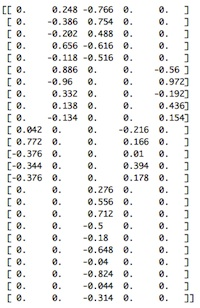
\includegraphics[width=.5\linewidth]{m_img}
	\caption{Group-wise sparse weight matrix generated: 5 classes, 25 features in 5 groups}
\end{center}
\end{figure}

Then we generate random vectors, each of which has a length of the number of all features, and calculate dot product with the weight matrix W to get the class assignments for these random vectors. The random vetors X and the class assignments Y make up the training data set. \\

Our goal is to infer this weight matrix W from X and Y using our model. By generating the data set using this method, we can test the effectiveness of our model on a noiseless dataset with right underlying assumptions.\\ 


\section{Results}

\subsection{Newsgroup Data}

Given limited resources, in our experiments we randomly select 200 articles from 3 news groups as the training data set. The selected articles are pre-processed to remove invalid words, stop words, low-frequency words. The co-occurence matrix method is used to generates groups. The maximal number of features in a group is set to 10. There are 37 groups created from the training data set. Then, all the features are re-ordered so that those belong to the same group are next to each other. The training vectors are aslo transformed to match the re-ordered features.\\  

The resulting weight matrix recoved is shown partically as below. The accuracy of the prediction is 93\%. The sparsity of the matrix is 52\% and the matrix is group-wise sparse.\\

\begin{figure}[ht]
  \centering
  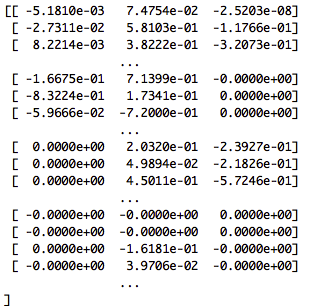
\includegraphics[width=\linewidth]{m4_img}
  \caption{Part of the Weight matrix computed from 200 articles from 3 topics. Each column is one topic class. Each row is a feature/word.}
\end{figure}%


\subsection{Artificial Data}

Shape Recovery. One of the main indicator of the effectiveness of our model is to see whether the calculated weight matrix is sparse group-wise. Our experiments show so. The following figures shows in a typical trial, the generated target weight matrix and the recovered weight matrix by our model. By comparing them side by side, we can tell that their sparsity patterns are similar. 


\begin{figure}[ht]
  \centering
  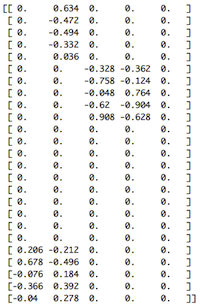
\includegraphics[width=.5\linewidth]{m1_img}
  \caption{Target group-wise sparse weight matrix generated: 5 classes, 25 features in 5 groups}
\end{figure}%

\begin{figure}[ht]
  \centering
  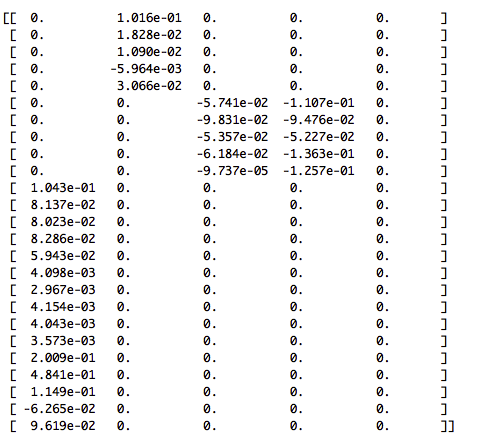
\includegraphics[width=.9\linewidth]{m2_img}
  \caption{Weight matrix calculated from the training data. It's similar to the one generated.}
\end{figure}


The different weights between the calculated matrix and the target matrix can be due to many factors. First, sample coverage is a major factor. In our simulation data, the sample size is small. Limited by the time complexity of the algorithm, it's difficult to complete the computation for a very large sample size in a reasonable time. Also, the sampling is random. There is no guaranteed that the inferred weights leads to the target weights. \\   

Accuracy. In our experiments, the generator algorithm was configured to produce 150 random vectors from the underlying model where it consists of 5 classes and 25 features in 5 groups. The accuracy achieved is closely related to the L2-norm regularization constant $\lambda$. The following figure shows the relation between lambda-accuracy and lambda-density.\\

\begin{figure}[ht]
\begin{center}
	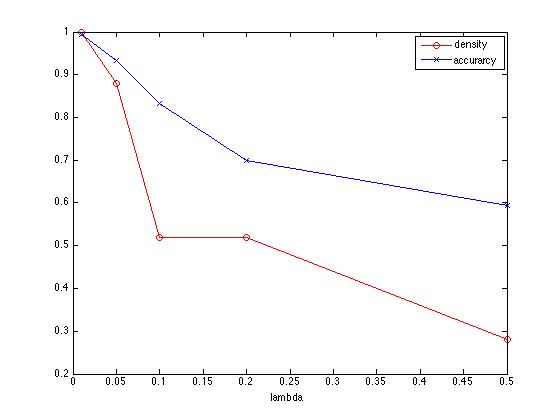
\includegraphics[width=\linewidth]{m3_img}
	\caption{lambda-accuracy and lambda-density plot (150 samples, 5 classes, 25 features in 5 groups)}
\end{center}
\end{figure}




\section{Conclusion}
% include your own bib file like this:
\bibliographystyle{acl}
\bibliography{ref}

\end{document}
